\documentclass{article}

\usepackage[table]{xcolor}
\usepackage{tabularx}
\usepackage{qtree}
\usepackage{color, colortbl}
\usepackage{amsmath}
\usepackage{tikz}
\usepackage{pgfplots}

\title{equations}
\author{}


\begin{document}
	\maketitle
	
	\begin{equation}
		\begin{array}{rl}
			pv(i, j) = \left\{ 
			\begin{array}{rl}
				max(x_{i - 1, j}, x_{i, j - 1})                & , x_{i - 1, j - 1} \leq min(x_{i - 1, j}, x_{i, j - 1}) \\
				min(x_{i - 1, j}, x_{i, j - 1})                & , x_{i - 1, j - 1} \geq max(x_{i - 1, j}, x_{i, j - 1}) \\
				x_{i - 1, j} + x_{i, j - 1} - x_{i - 1, j - 1} & ,  \textrm{otherwise}
			\end{array} \right.
			& , \textrm{where } 1 \leq i < \textrm{image height}, 1 \leq j < \textrm{image width}
		\end{array}
	\end{equation}
	
	
	\begin{equation}
		pv(i, j) = \left\{ 
		\begin{array}{rl}
			max(x_{i - 1, j}, x_{i, j - 1})                & , x_{i - 1, j - 1} \leq min(x_{i - 1, j}, x_{i, j - 1}) \\
			min(x_{i - 1, j}, x_{i, j - 1})                & , x_{i - 1, j - 1} \geq max(x_{i - 1, j}, x_{i, j - 1}) \\
			x_{i - 1, j} + x_{i, j - 1} - x_{i - 1, j - 1} & ,  \textrm{otherwise}
		\end{array} \right.
	\end{equation}
	
	\begin{equation}
		pe(i, j) = pv(i, j) \oplus pixel(i, j), \textrm{where } 1 \leq i < \textrm{image height}, 1 \leq j < \textrm{image width}
	\end{equation}
	
	\begin{equation}
		label(i, j) = \left\{ 
		\begin{array}{ll}
			8                       & , pe(i, j) = 0       \\
			7 - log_2(pe(i, j)) + 1 & , \textrm{otherwise}
		\end{array} \right.
	\end{equation}
	
	\begin{table}
		\caption{text}
		\centering
		\begin{tabular}{|c | c |}
			\hline 
			$x_1$ & $x_2$ \\
			\hline 
			$x_3$ & $x$   \\
			\hline 
		\end{tabular}
	\end{table}
	
	
	\begin{figure}
		\centering
		\begin{tabular}{|c | c |c | c |c | c |} \hline
			$x_{0, 0}$ & $x_{0, 1}$ & $x_{0, 2}$                         & $\dots$                           & $\dots$ & $x_{0, m}$ \\ \hline
			$x_{1, 0}$ & $\dots$    & $\dots$                            & $\dots$                           & $\dots$ & $\dots$    \\ \hline 
			$x_{2, 0}$ & $\dots$    & \cellcolor{blue!10} $x_{i-1, j-1}$ & \cellcolor{blue!10}$x_{i - 1, j}$ & $\dots$ & $\dots$    \\ \hline 
			$\dots$    & $\dots$    & \cellcolor{blue!10}$x_{i, j - 1}$  & \cellcolor{blue!10}$x_{i, j}$     & $\dots$ & $\dots$    \\ \hline 
			$x_{n, 0}$ & $\dots$    & $\dots$                            & $\dots$                           & $\dots$ & $x_{n, m}$ \\ \hline 
		\end{tabular}
		\caption{text}
	\end{figure}
	
	\begin{figure}
		\centering
		\begin{tabular}{|c | c |c | c |c | c |} \hline
			\rowcolor{lightgray}
			\cellcolor{lightgray}$N/A$   & $N/A$       & $\dots$     & $\dots$                        & $\dots$ & $N/A$       \\ \hline
			\cellcolor{lightgray}$N/A$   & $pv_{1, 1}$ & $pv_{1, 2}$ & $\dots$                        & $\dots$ & $pv_{1, m}$ \\ \hline
			\cellcolor{lightgray}$N/A$   & $pv_{2, 1}$ & $\dots$     & $\dots$                        & $\dots$ & $\dots$     \\ \hline 
			\cellcolor{lightgray}$\dots$ & $\dots$     & $\dots$     & $\dots$                        & $\dots$ & $\dots$     \\ \hline 
			\cellcolor{lightgray}$\dots$ & $\dots$     & $\dots$     & \cellcolor{blue!10}$pv_{i, j}$ & $\dots$ & $\dots$     \\ \hline 
			\cellcolor{lightgray}$N/A$   & $pv_{n, 1}$ & $\dots$     & $\dots$                        & $\dots$ & $pv_{n, m}$ \\ \hline 
		\end{tabular}
		\caption{text}
	\end{figure}
	
	
	
	\begin{figure}
		\centering
		\begin{tabular}{|p{.25 \textwidth} | p{.25 \textwidth} |p{.25 \textwidth} | p{.25 \textwidth} |}
			\hline 
			32 bits of Huffman coding rule & 20 bits of the length of the Huffman encoded label map & Huffman encoded label map & 1023 bytes of reference bytes \\ 
			\hline
		\end{tabular}
		\caption{text}
	\end{figure}
	
	\begin{figure}
		\centering
		\begin{tabular}{|p{.20 \textwidth} | p{.20 \textwidth} |p{.20 \textwidth} | p{.20 \textwidth}| p{.20 \textwidth} |}
			\hline 
			17 bits of Huffman coding tree topology & 36 bits of Huffman coding value & 20 bits of the length of the Huffman encoded label map & Huffman encoded label map & 16 bytes of reference bytes \\ 
			\hline
		\end{tabular}
		\caption{text}
	\end{figure}
	
	\begin{figure}
		\centering
		\Tree[.$\diamond$ [.$\diamond$ [.$\bullet$ \textit{00} ]
		[.$\bullet$ \textit{01} ]]
		[.$\diamond$ [.$\diamond$ [.$\bullet$ \textit{100} ] [.$\bullet$ \textit{101} ]  ]
		[.$\diamond$ [.$\diamond$ [.$\bullet$ \textit{1100} ] [.$\bullet$ \textit{1101} ]  ]
		[.$\diamond$ [.$\bullet$ \textit{1110} ]
		[.$\diamond$ [.$\bullet$ \textit{11110} ]
		[.$\bullet$ \textit{11111} ]]]]]]
		\caption{text}
	\end{figure}
	
	\begin{figure}
		\centering
		\Tree[.$\diamond$ [.0 [.0 00 ]
		[.1 01 ]]
		[.1 [.0 [.0 100 ] [.1 101 ] ]
		[.1 [.0 [.0 1100 ] [.1 1101 ] ]
		[.1 [.0 1110 ]
		[.1 [.0 11110 ]
		[.1 11111 ]]]]]]
		\caption{text}
	\end{figure}
	
	\begin{figure}
		\centering
		\Tree[.$\diamond$ [.$\diamond$ [.$\bullet$ \textit{00} ]
		[.$\diamond$ [.$\bullet$ \textit{010} ] [.$\bullet$ \textit{011} ]]]
		[.$\diamond$ [.$\diamond$ [.$\bullet$ \textit{100} ]
		[.$\diamond$ [.$\bullet$ \textit{1010} ]
		[.$\diamond$ [.$\bullet$ \textit{10110} ] [.$\bullet$ \textit{10111} ]]]  ]
		[.$\diamond$ [.$\bullet$ \textit{110} ] [.$\bullet$ \textit{111} ] ]]]
		\caption{text}
	\end{figure}
	
	\begin{figure}
		\centering
		\Tree[.$\diamond$ [.0 [.0 00 ]
		[.1 [.0 010 ] [.1 011 ]]]
		[.1 [.0 [.0 100 ]
		[.1 [.0 1010 ]
		[.1 [.0 10110 ] [.1 10111 ]]]]
		[.1 [.0 110 ] [.1 111 ]]]]
		\caption{text}
	\end{figure}
	
	\begin{equation}
		LM = \sum_{t=0}^{8} (freq[t] \times \textrm{the length of Huffman code of }t)
	\end{equation}
	
	\begin{figure}
		\centering
		
		\begin{tabular}{rl}
			$x_e = $         & 
			\begin{tabular}{| c | c | c | c | c | c | c | c |}
				\hline
				\cellcolor{lightgray}0 & \cellcolor{lightgray}0 & \cellcolor{lightgray}1 & \cellcolor{gray}1 & 0 & 1 & 0 & 1 \\
				\hline
			\end{tabular} \\
			
			& 
			\begin{tabular}{ c  c  c  c  c  c  c  c }
				\phantom{0} & \phantom{0} & $t = 3$ & \phantom{0} & \phantom{0} & \phantom{0} & \phantom{0} & \phantom{0} \\
			\end{tabular} \\
			
			secret bits =    & 
			\begin{tabular}{| c | c | c | c | c  c  c  c }
				\hline
				1 & 1 & 0 & 1 \\
				\hline
			\end{tabular} \\
			\phantom{0}      &         \\
			${x_e}\prime = $ & 
			\begin{tabular}{| c | c | c | c | c | c | c | c |}
				\hline
				\cellcolor{lightgray}1 & \cellcolor{lightgray}1 & \cellcolor{lightgray}0 & \cellcolor{gray}1 & 0 & 1 & 0 & 1 \\
				\hline
			\end{tabular}
		\end{tabular}
		
		
		\caption{text}
	\end{figure}
	
	\verb|<<|
	
	\begin{equation}
		{x_e}\prime(i, j) = \left\{
		\begin{array}{rl}
			x_e(i, j) \mod {2^{7-t}} + \sum_{s=0}^t(b_s \times 2^{7-s}) & , 0 \leq t < 7    \\
			\sum_{s=1}^8(b_s \times 2^{8-s})                            & , 7 \leq t \leq 8
		\end{array}
		\right.
	\end{equation}

	\begin{equation}
		x(i, j) = \left\{
		\begin{array}{ll}
			px(i, j) / {2^{7-t}} + b_{t+1} \times 2^{7-t} + x_{ew}(i, j) \mod {2^{7-t}} & , 0 \leq t < 8    \\
			px(i, j)                            & ,  t = 8
		\end{array}
		\right.
	\end{equation}

	\begin{equation}
		\begin{array}{rcl}
			MSB(x, b) & = & x ~\&~  (((1 \ll b) - 1) \ll (8 - b))  \\
			LSB(x, b) & = & x ~\&~  ((1 \ll b) - 1)
		\end{array}
	\end{equation}
	
	
	
	\begin{tabular}{| c | c | c | c | c | c | c | c | c | c |} \hline
		\rowcolor{lightgray}
		$t$       & 0    & 1    & 2     & 3     & 4     & 5     & 6     & 7     & 8     \\ \hline
		$freq(t)$ & 9818 & 9742 & 15247 & 33246 & 44509 & 53359 & 41758 & 24353 & 29089 \\ \hline
	\end{tabular}
	
	\phantom{0}
	
	\begin{tabular}{| c | c | c | c | c | c | c | c | c | c |} \hline
		\rowcolor{lightgray}
		$freq(t)$            & 9742                 & 9818                 & 15247                & 24353                & 29089 & 33246 & 41758 & 44509 & 53359 \\ \hline
		tree
		& \Tree[. [.1 ] ]  
		& \Tree[. [.0 ] ]  
		& \Tree[. [.2 ] ] 
		& \Tree[. [.7 ] ] 
		& \Tree[. [.8 ] ] 
		& \Tree[. [.3 ] ] 
		& \Tree[. [.6 ] ] 
		& \Tree[. [.4 ] ] 
		& \Tree[. [.5 ] ]      \\
		\hline
	\end{tabular}
	
	\begin{tabular}{| c | c | c | c | c | c | c | c | c |} \hline
		\rowcolor{lightgray}
		$freq(t)$ & 15247                                              & 19560 & 24353 & 29089 & 33246 & 41758 & 44509 & 53359 \\ \hline
		tree 
		& \Tree[. [.2 ] ]
		& \Tree[. [.9742 [.1 ]] [.9818 [.0 ] ] ]
		& \Tree[. [.7 ] ]
		& \Tree[. [.8 ] ]
		& \Tree[. [.3 ] ]
		& \Tree[. [.6 ] ]
		& \Tree[. [.4 ] ]
		& \Tree[. [.5 ] ]                                                                                       \\
		\hline
	\end{tabular}
	
	\begin{tabular}{| c | c | c | c | c  | c | c | c |} \hline
		\rowcolor{lightgray}
		$freq(t)$ & 24353 & 29089 & 33246 & 34807 & 41758 & 44509 & 53359 \\ \hline
		tree
		& \Tree[. [.7 ] ]
		& \Tree[. [.8 ] ]
		& \Tree[. [.3 ] ]
		& \Tree[. [.15247 [.2 ] ] [.19546  [.9742 [.1 ]] [.9818 [.0 ] ] ]]
		& \Tree[. [.6 ] ]
		& \Tree[. [.4 ] ]
		& \Tree[. [.5 ] ]   \\
		\hline
	\end{tabular}
	
	\begin{tabular}{| c  | c | c | c  | c | c | c |} \hline
		\rowcolor{lightgray}
		$freq(t)$   & 33246 & 34807 & 41758 & 44509 & 53359& 53442 \\ \hline
		tree
		& \Tree[. [.3 ] ]
		& \Tree[. [.15247 [.2 ] ] [.19546  [.9742 [.1 ]] [.9818 [.0 ] ] ]]
		& \Tree[. [.6 ] ]
		& \Tree[. [.4 ] ]
		& \Tree[. [.5 ] ]
		& \Tree[. [.24353 [.7 ] ] [.29089 [.8 ] ] ]   \\
		\hline
	\end{tabular}
	
	\begin{tabular}{ | c | c | c  | c | c | c |} \hline
		\rowcolor{lightgray}
		$freq(t)$     & 41758 & 44509 & 53359& 53442& 68053 \\ \hline
		tree
		& \Tree[. [.6 ] ]
		& \Tree[. [.4 ] ]
		& \Tree[. [.5 ] ]
		& \Tree[. [.24353 [.7 ] ] [.29089 [.8 ] ] ]  
		& \Tree[. [.33246 [.3 ] ] [.34807 [.15247 [.2 ] ] [.19546  [.9742 [.1 ]] [.9818 [.0 ] ] ]]] \\
		\hline
	\end{tabular}
	
	\begin{tabular}{ | c | c  | c | c | c |} \hline
		\rowcolor{lightgray}
		$freq(t)$  & 53359& 53442& 68053 & 86267 \\ \hline
		tree
		& \Tree[. [.5 ] ]
		& \Tree[. [.24353 [.7 ] ] [.29089 [.8 ] ] ]  
		& \Tree[. [.33246 [.3 ] ] [.34807 [.15247 [.2 ] ] [.19546  [.9742 [.1 ]] [.9818 [.0 ] ] ]]] 
		& \Tree[. [.41758 [.6 ] ] [.44509 [.4 ] ]]
		\\
		\hline
	\end{tabular}
	
	\begin{tabular}{ | c  | c | c | c |} \hline
		\rowcolor{lightgray}
		$freq(t)$  & 68053 & 86267& 106801 \\ \hline
		tree
		& \Tree[. [.33246 [.3 ] ] [.34807 [.15247 [.2 ] ] [.19546  [.9742 [.1 ]] [.9818 [.0 ] ] ]]] 
		& \Tree[. [.41758 [.6 ] ] [.44509 [.4 ] ]]
		& \Tree[. [.53359 [.5 ] ] [.53442 [.24353 [.7 ] ] [.29089 [.8 ] ] ] ]
		\\
		\hline
	\end{tabular}
	
	\begin{tabular}{  | c | c | c |} \hline
		\rowcolor{lightgray}
		$freq(t)$   & 106801& 154320 \\ \hline
		tree
		& \Tree[. [.53359 [.5 ] ] [.53442 [.24353 [.7 ] ] [.29089 [.8 ] ] ] ]
		& \Tree[. [.68053 [.33246 [.3 ] ] [.34807 [.15247 [.2 ] ] [.19546  [.9742 [.1 ]] [.9818 [.0 ] ] ]]]  [.86267 [.41758 [.6 ] ] [.44509 [.4 ] ]]]
		\\
		\hline
	\end{tabular}
	
	\begin{tabular}{  | c | c |} \hline
		\rowcolor{lightgray}
		$freq(t)$   & 261121 \\ \hline
		tree
		& \Tree[. [.106801 [.53359 [.5 ] ] [.53442 [.24353 [.7 ] ] [.29089 [.8 ] ] ] ] [.154320 [.68053 [.33246 [.3 ] ] [.34807 [.15247 [.2 ] ] [.19546  [.9742 [.1 ]] [.9818 [.0 ] ] ]]]  [.86267 [.41758 [.6 ] ] [.44509 [.4 ] ]]]]
		\\
		\hline
	\end{tabular}
	
	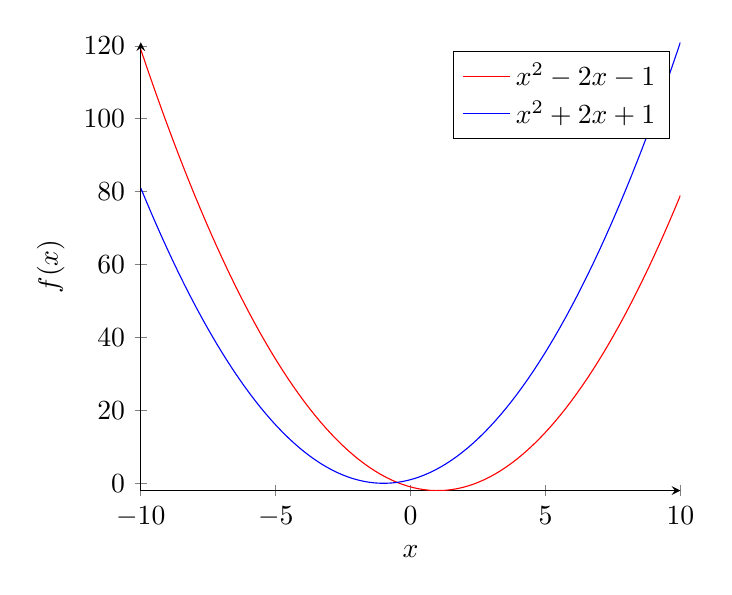
\begin{tikzpicture}
		\begin{axis}[
			axis lines = left,
			xlabel = \(x\),
			ylabel = {\(f(x)\)},
			]
			%Below the red parabola is defined
			\addplot [
			domain=-10:10, 
			samples=100, 
			color=red,
			]
			{x^2 - 2*x - 1};
			\addlegendentry{\(x^2 - 2x - 1\)}
			%Here the blue parabola is defined
			\addplot [
			domain=-10:10, 
			samples=100, 
			color=blue,
			]
			{x^2 + 2*x + 1};
			\addlegendentry{\(x^2 + 2x + 1\)}
			
		\end{axis}
	\end{tikzpicture}


	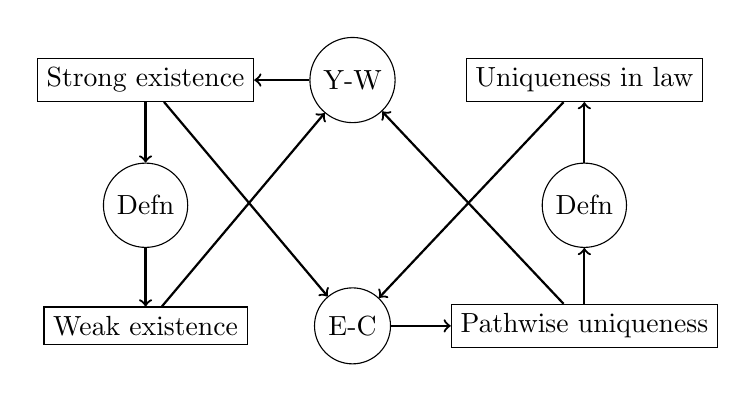
\begin{tikzpicture}
		\matrix [column sep=7mm, row sep=5mm] {
			\node (se) [draw, shape=rectangle] {Strong existence}; &
			\node (yw) [draw, shape=circle] {Y-W}; &
			\node (ul) [draw, shape=rectangle] {Uniqueness in law}; \\
			\node (d1) [draw, shape=circle] {Defn}; & &
			\node (d2) [draw, shape=circle] {Defn}; \\
			\node (we) [draw, shape=rectangle] {Weak existence}; &
			\node (ec) [draw, shape=circle] {E-C}; &
			\node (pu) [draw, shape=rectangle] {Pathwise uniqueness}; \\
		};
		\draw[->, thick] (se) -- (d1);
		\draw[->, thick] (d1) -- (we);
		\draw[->, thick] (we) -- (yw);
		\draw[->, thick] (yw) -- (se);
		\draw[->, thick] (se) -- (ec);
		\draw[->, thick] (ul) -- (ec);
		\draw[->, thick] (ec) -- (pu);
		\draw[->, thick] (pu) -- (yw);
		\draw[->, thick] (pu) -- (d2);
		\draw[->, thick] (d2) -- (ul);
	\end{tikzpicture}

	\begin{table}
		\centering
		\caption{text}
		\begin{tabular}{|c|c|c|c|c|} \hline
			Test Image & Total EC & LM & Extra bits & Net Payload \\ \hline
			Lena & 1470568 & 793304 & 52 & 2.583 \\ 
			Baboon & 1074384 & 794941 & 52 & 1.066\\
			Jetplane & 1587880 & 793441 & 52 & 3.030\\
			Man  \\
			Airplane & 1659203 & 682803 & 52 &3.724 \\
			Tiffany & 1526934 & 786527 & 52 & 2.824\\
		\end{tabular}
	
	\end{table}
	
\end{document}